\documentclass[10pt]{article}

\usepackage{fancyhdr}
\usepackage{graphicx}
\usepackage{ctex}
\usepackage[colorlinks,linkcolor=black]{hyperref}
\usepackage{xcolor}
\usepackage{listings}
\usepackage{geometry}


\lstset{
    numbers=left, 
    numberstyle= \tiny, 
    keywordstyle= \color{ blue!70},
    commentstyle= \color{red!50!green!50!blue!50}, 
    frame=shadowbox, % 阴影效果
    rulesepcolor= \color{ red!20!green!20!blue!20} ,
    escapeinside=``, % 英文分号中可写入中文
    xleftmargin=2em,xrightmargin=2em, aboveskip=1em,
    framexleftmargin=2em
} 


\newcommand\figcaption{\def\@captype{figure}\caption}
\newcommand\tabcaption{\def\@captype{table}\caption}


\pagestyle{fancy}
\lhead{《并行计算》实验报告}
\rhead{严愉程}

\makeatletter % 设置双线页眉
\def\headrule{{\if@fancyplain\let\headrulewidth\plainheadrulewidth\fi%
\hrule\@height 1.0pt \@width\headwidth\vskip1pt%上面线为1pt粗
%\hrule\@height 0.5pt\@width\headwidth  %下面0.5pt粗
\vskip-2\headrulewidth\vskip-1pt}      %两条线的距离1pt
\vspace{2mm}}     %双线与下面正文之间的垂直间距
\makeatother

% 版面布局控制
\baselineskip=15pt % 控制行距
\textheight 225mm  % 整个页面版芯的高度
\oddsidemargin 5.6mm
\evensidemargin 5.6mm
\parindent=2\ccwd  % 首行缩进的长度
\topmargin -5mm

\begin{document}

\begin{titlepage}
    \heiti
    \vspace*{64pt}
    \begin{center}
        \fontsize{56pt}{0} 西北工业大学\\
        \vspace*{36pt}
        \fontsize{48pt}{0}{实\quad 验\quad 报\quad 告}\\
        \vspace*{48pt}
        \LARGE(2020\~{}2021学年 秋季学期)\\
        \vspace*{48pt}
    
        \LARGE 课程名称\ \ \ \underline{\makebox[140pt]{《并行计算》}}\\
        \vspace*{72pt}
    
        \Large 姓名\ \ \underline{\makebox[108pt]{严愉程}}\\
        \Large 学号\ \ \underline{\makebox[108pt]{2017300138}}\\
        \Large 学院\ \ \underline{\makebox[108pt]{教育实验学院}}\\
        \Large 班级\ \ \underline{\makebox[108pt]{HC001706}}\\
        \Large 专业\ \ \underline{\makebox[108pt]{计算机科学与技术}}\\
    \end{center}
\end{titlepage}

\tableofcontents

\title{\bf\Large 《并行计算》实验报告}
\date{2020/12/30}
\author{\small 严愉程}
\maketitle

\thispagestyle{fancy}

\section{实验目的}

1.熟悉MPI编程环境,掌握MPI编程基本函数及MPI的相关通信函数用法,掌握MPI的主从模式及对等模式编程;

2.熟悉OpenMP编程环境,初步掌握基于OpenMP的多线程应用程序开发,掌握OpenMP相关函数以及数据作用域机制、多线程同步机制等。 

\section{实验环境}
ubuntu18.04,inteli7-7700HK 4核8线程,gcc8.2,OpenMPI 4.2.0。使用CMake构建。

\section{实验内容}
分别进行以下实验:1.用Monte-Carlo随机积分算法估算$\pi$值的并行算法;2.Floyd算法的并行化;3.N皇后问题并行算法

\subsection{Monte-Carlo随机积分算法估算$\pi$值的并行算法}

\subsubsection{算法原理}

算法的原理比较简单,在第一象限上的单位正方形内随机放点,落在单位圆内的点的个数 / 点的总个数 = $\pi$ / 4。

多个线程并行的进行多次投掷,然后reduce到一个线程上。

\subsubsection{实验步骤}
(1)写CMakelists,配置编译环境

(2)编写代码主要有几个模块:
\quad 1.随机数生成模块,需要阻止每个线程生成相同的随机数序列 \\
\quad 2.为了保证运算精度我用了大数运算的库(受限于电脑性能,我最后没到达那个精度) \\
\quad 3.主线程进行reduce求和 \\


\subsubsection{运行结果}

运行结果如图\ref{pi结果图}所示。

\begin{figure}[htbp]
    \centering
    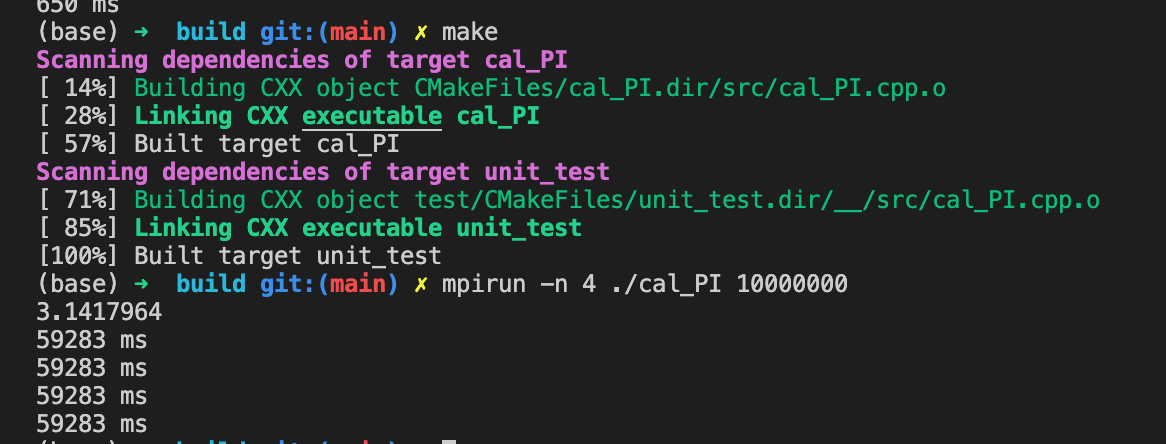
\includegraphics[width=.6\textwidth]{assets/cal_PI.png}
    \caption{计算$\pi$值算法的运行结果图}
    \label{pi结果图}
\end{figure}

\subsubsection{算法分析}

\begin{table}[htbp]
    \centering
    \caption{并行计算$\pi$运行结果}
        \begin{tabular}{|c|c|c|c|c|c|}
        \hline
          &  & \multicolumn{2}{|c|}{线程为2} & \multicolumn{2}{|c|}{线程为4} \\ \cline{3-6}
        模拟次数 & 线程数为1的运行时间 & 运行时间 & 加速比 & 运行时间 & 加速比 \\
        \hline
        1000000 & 12287 ms & 7508 ms & 1.636 & 5825 ms & 2.109 \\
        \hline
        5000000 & 69005 ms & 40313 ms & 1.711 & 30667 mss & 2.250 \\
        \hline
        \end{tabular}
    \label{pi_table}
\end{table}

\paragraph{并行性能分析}

算法随不同n和p的值性能如表\ref{pi_table}所示。随着数据量的增加,加速比有所提高。

\paragraph{算法可扩展性分析}

算法对处理器上限没有要求,随着处理器的个数增多,可以扩大问题的计算范围$\pi$的精度也会有所提高。

\subsection{Floyd并行算法}

\subsubsection{算法原理}

\paragraph{floyd串行的原理}

\begin{figure}[htbp]
    \centering
    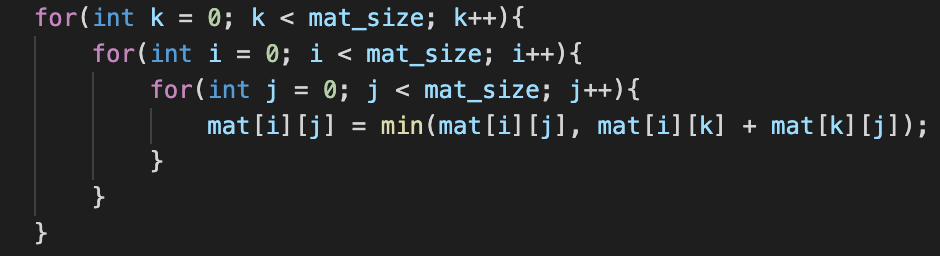
\includegraphics[width=.6\textwidth]{assets/floyd串行.png}
    \caption{floyd串行代码}
    \label{floyd串行代码}
\end{figure}

串行版代码比较简单,见图\ref{floyd串行代码},采用了动态规划的思想。

最外层的k就是考虑以节点k为中转点,尝试节点i到节点j通过节点k的中转,能否更近。

第k次迭代的含义是,在尝试过前面k-1个节点作为中转点的基础上,尝试节点k作为中转点,求任意两点之间的最短路。迭代最后会最后尝试遍所有中转点。

\paragraph{并行的设计思路} 

根据四步设计法:

(1)划分:算法对$mat[i][j] = \min(mat[i][j], mat[i][k] + mat[k][j])$ 进行了$n^{3}$次操作。可以把矩阵$mat[][]$上的$n^{2}$个元素作为一个原子任务。

(2)通信:每个任务在第k次迭代的时候,需要知道$mat[i][k]$和$mat[k][j]$。

(3)聚合:每个原子任务都有相似的计算时间,我们在聚合的时候考虑通讯量。

读取矩阵的时候是按行读取的,自然采用按行聚合的方式。而且按行聚合不需要通讯$mat[i][k]$,只需要通讯$mat[k][j]$,即,在k次迭代之前,通讯k行。

(4)映射:按行,分组映射到每个处理器即可。最后一个处理器来处理余下的部分,并进行矩阵的读取与发送,作为master线程。


\subsubsection{实验步骤}

(1)写CMakelists.txt。准备编译环境。

(2)编写并行的floyd代码。首先进行矩阵的读取,然后计算,然后master线程,通过send,recv的形式控制线程依次写结果。

(3)写验证用的串行floyd代码。验证结果正确。

第一版的算法,在通讯的手段上比较粗糙,随着最外层变量k的迭代过程中,每一次矩阵mat[][]更新都进行一次矩阵的同步,即每个线程都广播一次自己管辖的矩阵区域,如图\ref{floyd代码第一版的运行结果}。在$mat_size=4000$的节点数下,多线程的运行时间和单线程的差不多,虽然能够得出正确的结果,但加速比不理想。

\begin{figure}[htbp]
    \centering
    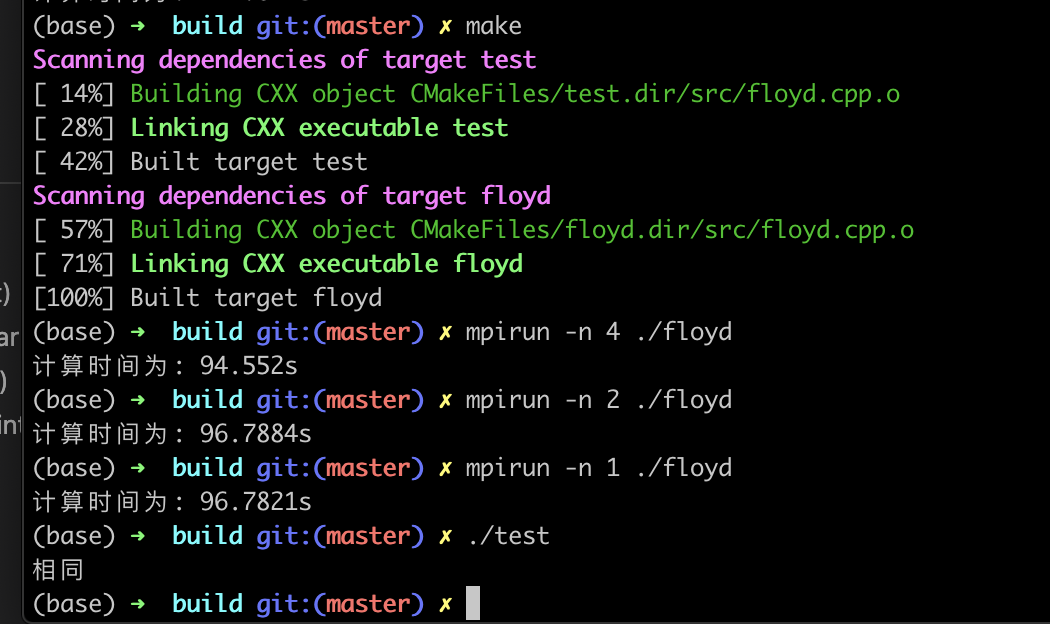
\includegraphics[width=.6\textwidth]{assets/floyd命令行运行界面.png}
    \caption{floyd代码第一版的运行结果}
    \label{floyd代码第一版的运行结果}
\end{figure}

考虑从通信量上的进行优化。在操作$mat[i][j] = \min(mat[i][k] + mat[k][j])$中,最外层循环k迭代的时候,$mat[i][k]$的数据永远在本线程管辖的区域内,不需要同步。而$mat[k][j]$会随着k的迭代,出现其他线程管辖的区域或者本线程管辖的区域是不确定的。

所以每次k迭代的时候,各个线程需要的是k行数据,迭代k次之前要广播k行。

需要注意的是,每次迭代的时候,实际上每个线程管辖的区域都更新了,最后还需要把这些更新进行同步,因为题目要求的是线程依次按照顺序分别写入,就不需要进行同步(在多节点的系统上注意需要进行同步)。

改进之后的运行结果如图\ref{floyd优化版命令行运行结果}所示。

\subsubsection{运行结果}

\begin{figure}[htbp]
    \centering
    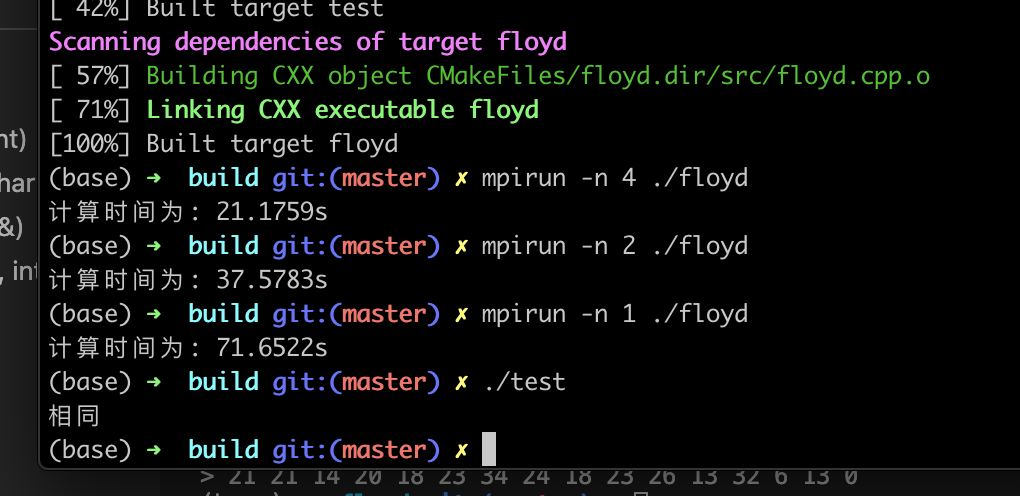
\includegraphics[width=.6\textwidth]{assets/floyd第二版命令行运行结果.png}
    \caption{floyd优化版命令行运行结果}
    \label{floyd优化版命令行运行结果}
\end{figure}

并行版的floyd算法与串行版的floyd算法运行结果相同,得出:并行版的floyd算法运行正确。且在节点个数为4000的问题规模下,线程个数为4时加速比3.384。

\subsubsection{算法分析}

\paragraph{并行性能分析}

不同线程个数和不同问题规模下,该算法的并行性能,如表\ref{floyd_table}所示。


\begin{table}[htbp]
    \centering
    \caption{floyd运行结果}
        \begin{tabular}{|c|c|c|c|c|c|}
        \hline
          &  & \multicolumn{2}{|c|}{线程为2} & \multicolumn{2}{|c|}{线程为1} \\ \cline{3-6}
        矩阵的大小 & 线程数为1的运行时间 & 运行时间 & 加速比 & 运行时间 & 加速比 \\
        \hline
        4000 & 71.6522s & 37.5783s & 1.907 & 21.1759s & 3.384 \\
        \hline
        2000 & 9.36538s & 5.47045s & 1.711 & 3.69849s & 2.536 \\
        \hline
        \end{tabular}
    \label{floyd_table}
\end{table}

\paragraph{算法可扩展性分析}

该算法是按照行来进行划分的,可以使用的处理器个数的上限为行的数量。如果有充足的处理器,可以考虑棋盘式划分的方法。
对于一个集群系统,在节点的内部还可以使用openmp进行并行。openmp相对于mpi更加时候统一内存架构,且在一定的情况下编程相对方便。

\begin{figure}[htbp]
    \centering
    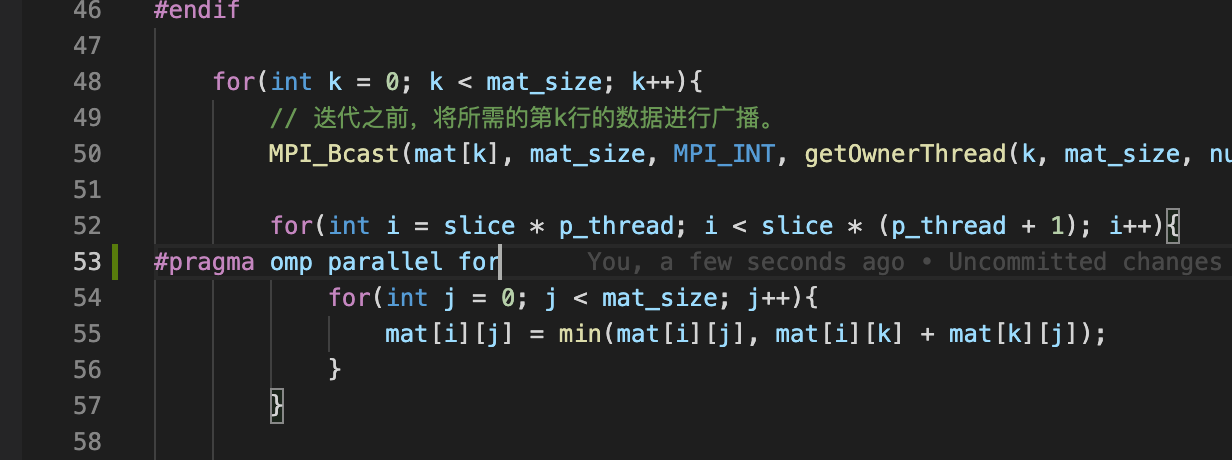
\includegraphics[width=.8\textwidth]{assets/openmp+MPI.png}
    \caption{使用openmp+MPI混合编程}
    \label{使用openmp+MPI混合编程}
\end{figure}

\subsection{超快速并行算法}

\subsubsection{算法原理}

我这里举一个8线程情况时候的例子,就比较容易理解算法原理。

(1)首先将数组平均分给8个线程。每个线程分别进行快速排序。这样就得到了8个有序子数组,下面分别用0, 1, 2, ..., 7来表示

(2)此时(0,1,2,3,4,5,6,7)在同一线程组中,0号线程将自己的中位数pivot广播。

(3)每个线程根据0号线程广播的pivot,将本线程中的子数组进行划分,分为大的一部分upper和小的一部分lower。

(4)0和4,1和5,2和6,3和7交换两个部分。比如,0号线程拿0和4中的lower,进行归并。4号线程拿0和4中的upper,进行归并

(5)结果就有,(0,1,2,3) < (4,5,6,7)中的元素,拆分成了两个线程组。对每个线程组重复步骤(2)到步骤(5)的操作

(6)结果依次有(0,1)< (2,3) < (4,5) < (6,7)

(7)最后有 (0) < (1) < (2)< (3)< (4)< (5) < (6)< (7)


\subsubsection{实验步骤}

按照上面的算法原理编写代码实现即可。


\subsubsection{运行结果}

\begin{figure}[htbp]
    \centering
    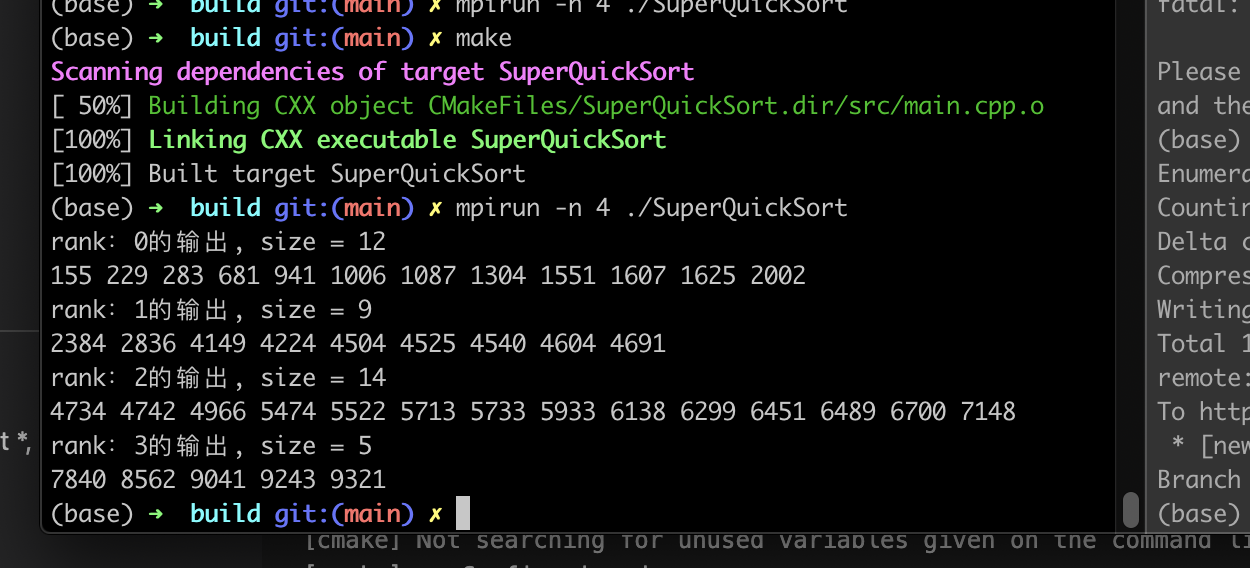
\includegraphics[width=.8\textwidth]{assets/SuperQuickSort.png}
    \caption{超快速并行排序命令行运行结果图}
    \label{超快速并行排序}
\end{figure}


\subsubsection{算法分析}

\paragraph{并行性能分析}

\begin{table}[htbp]
    \centering
    \caption{并行计算$\pi$运行结果}
        \begin{tabular}{|c|c|c|c|c|c|}
        \hline
          &  & \multicolumn{2}{|c|}{线程为2} & \multicolumn{2}{|c|}{线程为4} \\ \cline{3-6}
        模拟次数 & 线程数为1的运行时间 & 运行时间 & 加速比 & 运行时间 & 加速比 \\
        \hline
        1e6 & 0.28186s & 0.267679s & 1.053 & 0.259043s & 1.088 \\
        \hline
        1e7 & 2.76637s & 3.25229s & 0.852 & 3.14133s & 1.035 \\
        \hline
        \end{tabular}
    \label{pi_table}
\end{table}

很遗憾没能写出并行性能很好的算法,初步怀疑是IO数据量大的问题,或者我的代码没有优化好。


\paragraph{算法的可扩展性分析}

线程数的扩展能力较强。



\subsection{N皇后问题并行算法}

\subsubsection{算法原理}

算法比较简单,一个典型的DFS问题,可以在搜索的每个分之上进行并行。这里我使用openmp进行编程。

\subsubsection{运行结果}

\begin{figure}[htbp]
    \centering
    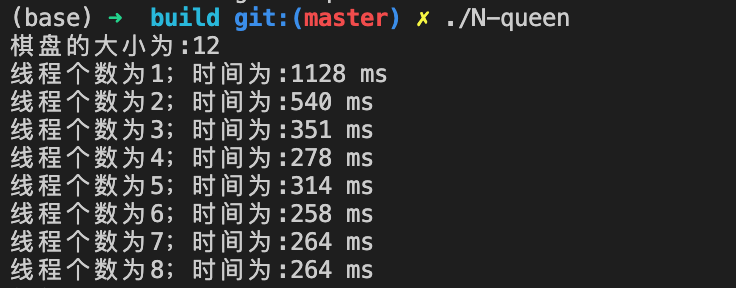
\includegraphics[width=.6\textwidth]{assets/n-queen-performance.png}
    \caption{N皇后程序运行截图}
    \label{N皇后程序运行截图}
\end{figure}

\subsubsection{算法分析}
分析不同n值、P值以及不同有序度时算法的运行时间,进行算法并行性能和可扩展性分析。(*)

\paragraph{并行性能分析}

\begin{table}[htbp]
    \centering
    \caption{棋盘大小为12时的性能}
        \begin{tabular}{c|c|c}
        \hline
        线程个数 & 计算所用时间(ms) & 加速比 \\
        1 & 1128ms & 1 \\
        2 & 540ms & 2.08 \\
        3 & 351ms & 3.21 \\
        4 & 278ms & 4.05 \\
        5 & 314ms & 3.59 \\
        6 & 258ms & 4.37 \\
        7 & 264ms & 4.27 \\
        8 & 264ms & 4.27 \\
        \end{tabular}
    \label{n-queen-performance}
\end{table}

\paragraph{算法的可扩展性分析}

目前算法扩展的线程上限数量为棋盘的大小。

\section{实验总结}

通过思考并行算法,以及编程实现,我在复习课堂上的基础知识的同时,也提升了我的动手能力。让我进一步掌握了,OpenMP、MPI这两个并行计算的工具,以及混合编程的优势。

\end{document}

